% \begin{unnecessary}
% \textbf{Слабая топология и слабая сходимость}

% \begin{definition}
%     $S$ называется \textit{секвенциально слабо замкнутым} (с.с.з) множеством, если
%     $$\forall \{x_n\}\subset S,\; n \in \N \;\; x_n \weakconv x
%     \implies x \in S.$$
% \end{definition}

% \begin{statement}
%     Секвенциальная слабая замкнутость $\implies$ замкнутость.
% \end{statement}

% Можно придумать топологию, порождающую слабую сходимость, но мы об этом не говорим. Рассмотрим разные виды замыканий:
%     \[\overline{S(0; 1)} \subset \overline{S(0; 1)}^{\text{ секв. сл.}} \subset \overline{S(0; 1)}^{\text{ сл.}}\]

%     Чем слабее топология, тем больше замыкание. Чем сильнее топология, тем проще отображению быть непрерывным.
% \end{unnecessary}

    \underline{Запас непрерывности у ограниченных линейных операторов:}
    
    Рассмотрим $E$ и класс линейных ограниченных отображений 
    $\mathcal{L}(E)$. $A \in \mathcal{L}(E)$~--- непрерывно по норме $\| \cdot \|$. А в слабой топологии? Просто по определению и следствиям останется непрерывным.
    \begin{theorem}  % нумерация лектора
        Пусть $E_1, E_2$~--- нормированные пространства, $A \in \mathcal{L}(E_1, E_2)$. Тогда из условия $x_n \weakconv x$ следует, что $Ax_n \weakconv Ax$.
    \end{theorem}
    \begin{proof}\textit{ Cогревающее душу.}\\
    \begin{figure}[H]
        \centering
        % 
\includegraphics[width=0.4\textwidth]{images/7_2.jpg}
        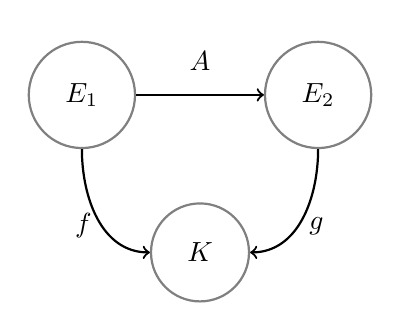
\begin{tikzpicture}[inner sep=3mm,thick]
            \node (field) at (0,0) [circle,draw=black!50] {\(\mathbb{K}\)};
            \node (E1) at (-1.5,2) [circle,draw=black!50] {\(E_1\)};
            \node (E2) at (1.5,2) [circle,draw=black!50] {\(E_2\)};
            \draw [->] (E1.east) to node[above] {\(A\)} (E2.west);
            \draw [->] (E1.south) to [out=270,in=180] node[below,anchor=center,yshift=-0.6ex,xshift=-1.2ex] {\(f\)} (field.west);
            \draw [->] (E2.south) to [out=270,in=0] node[below,anchor=center,yshift=-0.6ex,xshift=1.2ex] {\(g\)} (field.east);
        \end{tikzpicture}
    \end{figure}
    Пусть есть оператор $A\!\!:\! E_1 \to E_2$. Возьмём произвольный функционал $g \in E_2^*$. Рассмотрим отображение $f = g \circ A$~--- линейный непрерывный функционал (как суперпозиция). Тогда $f \in E_1^*$.

    Получаем, что по определению слабой сходимости
    \[\forall g \in E_2^* \;\;\; gA(x_n) \to gA(x)  \implies g(Ax_n) \to g(Ax) \implies  A x_n \weakconv Ax.\]
    \end{proof}
    
\begin{definition}
    Множество $S \subset E$, $E$~-- нормированное, называется \textit{слабо ограниченным}, если $\forall f \in E^* \: f[S]$~--- ограничено т.е. \[\forall f \in E^* \; \forall x \in S \left(|f(x)| \leq C(f) \right) \quad \text{(не зависит от $x$)}\]
\end{definition}

\begin{lemmanote}
    Сравним это определение с ограниченностью.

    $S$~-- ограничено, если $\exists C > 0\: \forall x \in S \left(\|x\|\leqslant C \right)$
\end{lemmanote}

\begin{theorem}[Хана]\label{han}
    Слабая ограниченность $\Leftrightarrow$ ограниченность
\end{theorem}

\begin{proof}
\begin{itemize}
    \item[$\Leftarrow$]
    \[\exists R\:\forall x \in S\left( \|x\| \leqslant R \right)\]
    Тогда \[|f(x)| \leqslant \|f\| \cdot \|x\| \leqslant \|f\| \cdot R = C(f)\]

    Следовательно, $S$~--- слабо ограничено.
    \item[$\Rightarrow$] Предположим противное, то есть $S$~--- слабо ограничено, но не ограничено. Тогда
    \[\forall n \in \N\; \exists x_n \in S \left(\;  \| x_n \| \geqslant n^2 \sim \frac1 n \| x_n \| > n \right)\]

    Рассмотрим $y_n = \frac 1 n x_n \weakconv 0$, так как $f(y_n) = f(\frac 1 n x_n ) =\frac{1}{n} f(x_n) \to 0$ в силу слабой ограниченности $x_n$. Откуда по критерию слабой сходимости~\ref{criteria_weak_to} $\{ \| \frac 1 n x_n \| \}$ --- ограничена, что противоречит выбору $x_n$.
\end{itemize}
\end{proof}

\begin{unnecessary}
\textbf{Слабая топология и слабая сходимость}
\begin{definition}
    $S$ называется \textit{секвенциально слабо замкнутым} (с.с.з) множеством, если
    $$\forall \{x_n\}\subset S,\; n \in \N \;\; x_n \weakconv x
    \implies x \in S.$$
\end{definition}

\begin{statement}
    Секвенциальная слабая замкнутость $\implies$ замкнутость.
\end{statement}

\begin{proof}
    Пусть $\|x_n - x\| \to 0, \: x_n \in S \implies x_n \weakconv x \underbrace{\implies}_{\text{условие}} x \in S$.
\end{proof}

\begin{statement}
    В гильбертовом пространстве замкнутость подпространства влечёт секвенциально слабую замкнутость (в произвольном пространстве и с произвольным множеством это неверно).\\
    Контрпример: (не подпространство) $S(0,1) \subset l_2$ 
\end{statement}

\begin{proof}
    Пусть $x_n \weakconv x,\; x_n \in L \sim (x_n,y) \to (x,y)$. Возьмём $y \in L^\perp$. Откуда получаем, что $0=(x_n,y) \to (x,y)=0$

    Следовательно, $x \in (L^\perp)^\perp = L.$
\end{proof}

\begin{definition}
    Последовательность $\{x_n\} \subset E$ называется \textit{слабо фундаментальной} если 
    \[\forall f\in E^*\;\; \{f(x_n)\}\text{~--- фундаментальна.}\]
\end{definition}

\begin{definition}
    Пространство является \textit{секвенциально полным}, если $\forall \{x_n\}$~--- слабо фундаментальна $\implies \{x_n\}$~--- слабо сходящаяся
\end{definition}

Пример не секвенциально полного пространства: $c_0$ (см. книгу Константинова), $C[a, b]$
\begin{statement}
    Любое гильбертово пространство является секвенциально слабо полным
\end{statement}

\begin{proof}
    см. задание
\end{proof}

\textbf{Какие есть сходимости в $E^*$:}
\begin{itemize}[noitemsep, topsep=1pt]
    \item[-] по норме
    \item[$\Downarrow$]
    \item[-] слабая сходимость (через $E^{**}$)
    \item[$\Downarrow$]
    \item[-] поточечная сходимость на элементах из $E$ в $E^*$ (*-слабая сходимость)
\end{itemize}


\begin{example}
    В $l_2$ шар $\overline{B(0, 1)}$~--- не компакт, но секв. слабый компакт \textit{(трудный факт)}.
\end{example}

\begin{definition}
    $S$~--- \textit{секвенциально слабо компактное}, если\\
    $\forall \{ x_n \} \subset S \; \exists$ слабо сходящаяся подпоследовательность $x_{n_k} \weakconv x \in S$.
\end{definition}

\end{unnecessary}